\begin{problem}
{\textbf{\textsc{An Envelope of Light}}} 
A point light source on the ceiling is located at the center of a cylindrical housing (with an open base) of radius $R$ and height $H$. A wall is a horizontal distance $D$ from the center of the cylinder. Now consider a coordinate system with the light source at the origin. The wall, at $x=-D$, has the following shape in the $y-z$ plane:

\begin{center}
    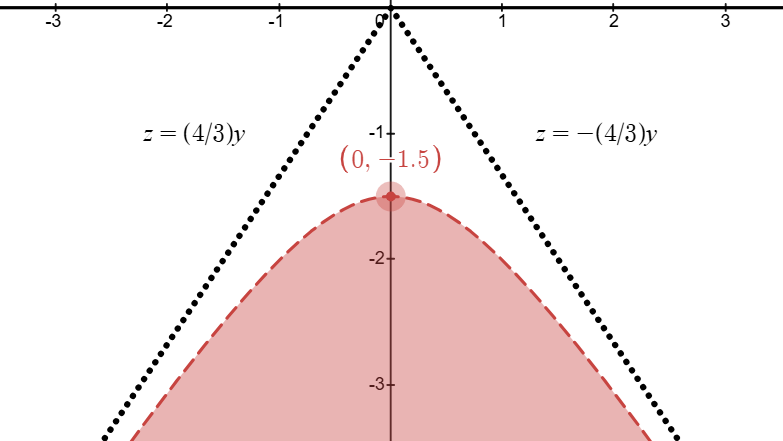
\includegraphics[height=0.3\textwidth]{problems/figures/lightConeGraph.png}
    \hspace{2em}
    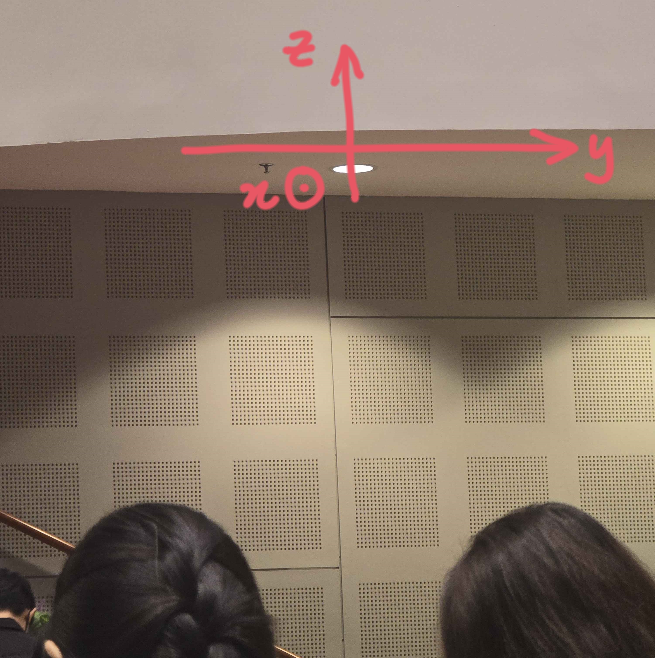
\includegraphics[height=0.3\textwidth]{problems/figures/lightConeHyperbola.png}
\end{center}

The vertical coordinate of the highest point of the curve observed is $-1.5\;\mathrm{m}$, while the gradients of the lines asymptotically tangent to the curve are $\pm 4/3$. On the right is shown an example setup of this phenomenon. Find the horizontal distance $D$ of the wall to the light source.
\end{problem}